\chapter{Research Plan}
\label{cha:research_plan}

As previously mentioned in Section~\ref{subsec:what_are_dna_sequences}, by looking at the sequence of a DNA segment, scientists can figure out what kind of genetic information it contains. 

For example, scientists can utilize sequence information to determine which stretches of DNA include genes and which stretches have regulatory instructions that turn genes on or off. This is achieved by finding a protein called \gls{TF} which are \gls{DBS} that bind target DNA to activate or suppress gene transcription and are involved in a variety of biological activities. The research of \gls{TF} function begins with accurate identification of \gls{TF}s~\cite{Hu2019AnimalTFDBFactors}.

It is also possible to explore the sequence data to identify essential genes. These are a group of genes that are required for a living organism's survival or reproduction~\cite{Zhang2020DeepHE:Learning}. Several wet-lab experimental approaches can be used to identify essential genes, however these procedures are frequently time-consuming, arduous, and expensive. Some classic machine learning-based approaches have been offered as a complement to the experimental methods, with the primary goal of predicting essential genes on model organisms~\cite{Zhang2020DeepHE:Learning}.

\begin{figure}[htbp]
    \centering
    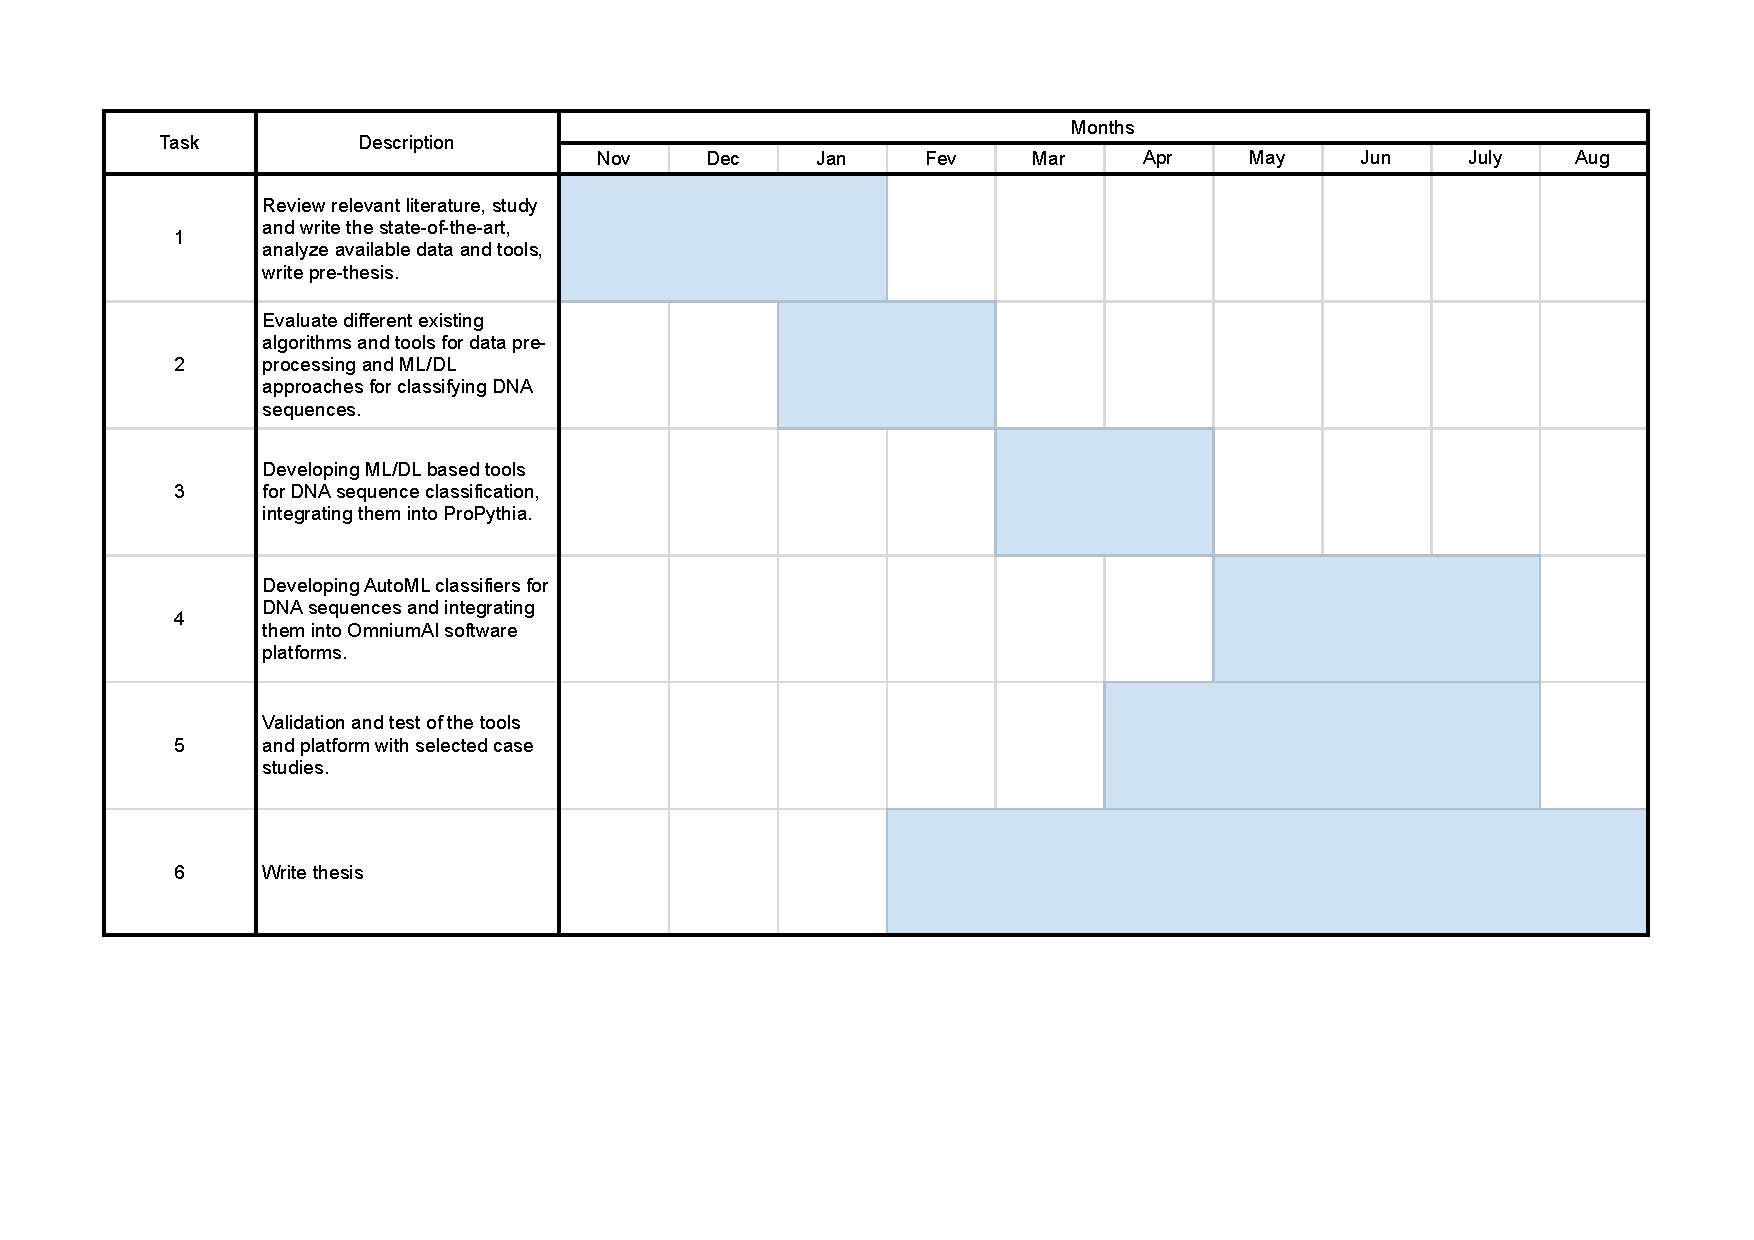
\includegraphics[width=\linewidth]{gantt.pdf}
    \caption{Thesis Gantt diagram}
    \label{fig:gantt}
\end{figure}